\documentclass[tikz]{standalone}

\definecolor{data color}{RGB}{200,10,200}
\definecolor{axis color}{RGB}{200,10,0}
\definecolor{accum color}{RGB}{0,150,10}
\definecolor{flow color}{RGB}{10,30,245}
\definecolor{flow fill}{RGB}{200, 215, 255}

\begin{document}
	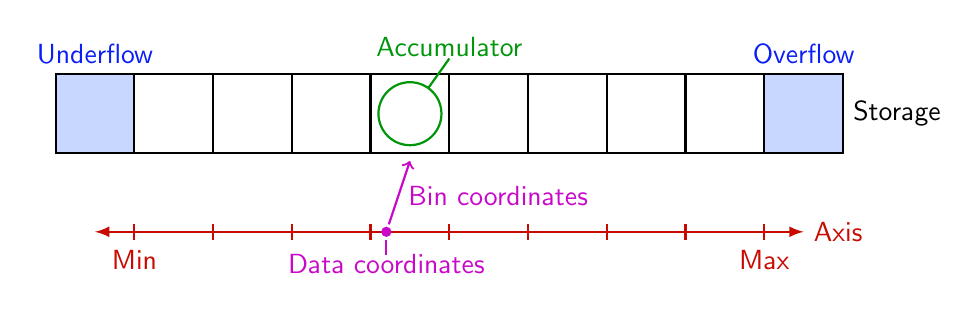
\begin{tikzpicture}[font=\sffamily, thick]
	\path [fill=flow fill] (0,0) rectangle (1,1);
	\path [fill=flow fill] (9,0) rectangle (10,1);
	\draw (0,0) rectangle (10,1);
    \foreach \x in {1,...,9}
    	\draw (\x,0) -- (\x, 1);
        
    \node at (.5, 1) [above, flow color] {Underflow};
    \node at (9.5, 1) [above, flow color] {Overflow};
    \node at (10, .5) [right] {Storage};
    
    \begin{scope}[axis color]
        \draw [latex-latex] (.5, -1) -- (9.5, -1);
	    \foreach \x in {1,...,9}
	        \draw (\x,-1.1) -- (\x, -.9);
	    
	    \node at (9.5, -1) [right] {Axis};
	    \node at (1, -1.1) [below] {Min};
	    \node at (9, -1.1) [below] {Max};
   \end{scope}
   
    \begin{scope}[data color]
	    \draw [->, shorten <=.1 cm] (4.2, -1) -- (4.5, -.1) node [midway, right] {Bin coordinates};
	    \draw [fill] (4.2, -1) circle (.05);
	    \draw (4.2, -1.1) -- (4.2, -1.3) node [below=-.15cm] {Data coordinates};
    \end{scope}
        
    \begin{scope}[accum color]
	    \draw (4.5, 0.5) circle (.4) ;
	    \draw [shorten <= .4 cm] (4.5, 0.5) -- (5, 1.2)  node [above=-.1cm] {Accumulator};
    \end{scope}
        
	\end{tikzpicture}
\end{document}